\documentclass[../main.tex]{subfiles}

\begin{document}
	\section{Einleitung}
	
	\subsection{Ausgangslage}
	Ein Aquaponics Projekt besteht bereits aus folgenden Komponenten. Sensoren der Aquaponics Systeme, welche an SC1000 Geräten angeschlossen sind. \\
	Ein serieller Bus verknüpft alle SC1000 mit einem RasPi welches über eine Modbus-API die Sensordaten auf eine MySQL Datenbank ablegt. Diese Daten werden auf der Webseite dargestellt. \\
	Die Webseite, welche unter myaquaculturefarm.ch zu finden ist, wird auf hosttech.ch gehostet. Hosttech verwendet als Backend Technologie PHP.\\
	Unsere Konfigurationsseite wird ebenfalls auf dieser Domain parallel zu den anderen Webseiten von ZHAW Life Sciences und Facility Management gehostet. \\
	Beim Backend sind wir gebunden was die Host-Firma uns zur Verfügung stellt, in diesem Falle wäre das PHP.
	
	\begin{figure}[H]
		\centering
		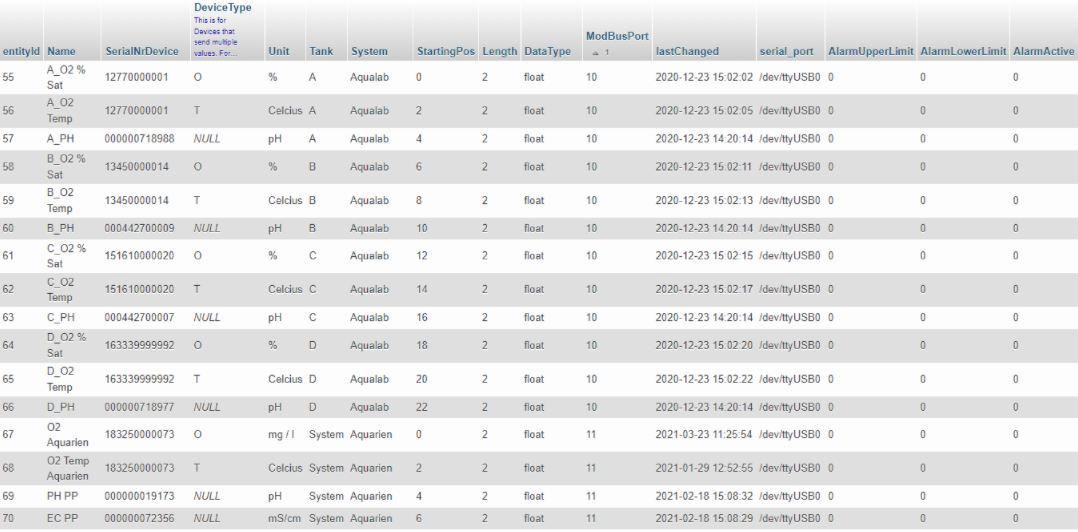
\includegraphics[scale=0.5]{Modbusentity}
		\caption{Modbusentity Tabelle}
		\label{fig:Modbusentity}
	\end{figure}
	\par \noindent
	Wie in der oberen Abbildung zu sehen ist werden die gesamten Sensorendaten in diese Tabelle eingespeist. Dadurch, dass es kein Interface gibt müssen die Daten jedesmal manuell in die Tabelle eingetragen werden. Falls es neue Tanks gibt benötigen sie eine neue Erkennungsnummer.  \\
	In der folgenden Abbildung werden die Daten geloggt um ein Archivierung älterer Daten zu ermöglichen.
	
	\begin{figure}[H]
		\centering
		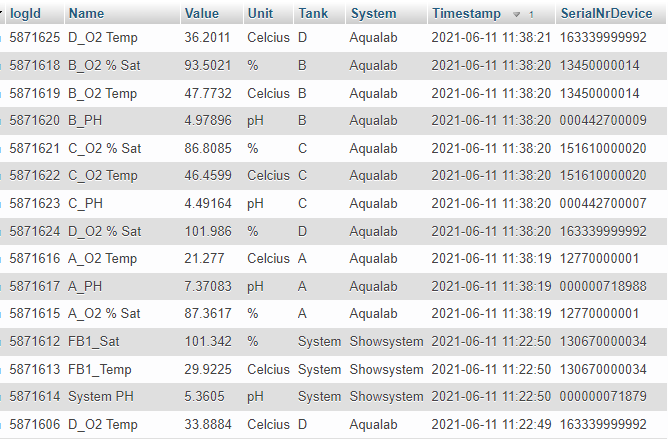
\includegraphics[scale=0.5]{Modbuslog}
		\caption{Modbuslog Tabelle}
		\label{fig:Modbuslog}
	\end{figure}
	\par \noindent	
	Um die Übersicht über die einzelnen Tanks zu wahren gibt es hier die Kolonnen Tank und Systeme, welche anzeigen woher die einzelnen Sensorendaten stammen.
	
	\subsection{Gesamtarchitektur}
	In den Becken befinden sich Sensoren die verschiedene Messungen führen. Alle Sensoren eines Systems hängen an einem SC1000 Gerät. Alle SC1000 Geräte sind mit dem Modbus verbunden. Über diesen Modbus holt sich das ein Raspberry Pi alle Sensordaten von allen Systemen und logt und ladet diese hoch auf eine MySQL Datenbank. Dass das Raspberry Pi auch weiss an welcher Adresse auf dem Mobdus welcher Sensor abgefragt werden kann, werden die Konfigurationen aller Systeme innerhalb der MySQL Datenbank gespeichert.
	\begin{figure}[h]
		\centering
		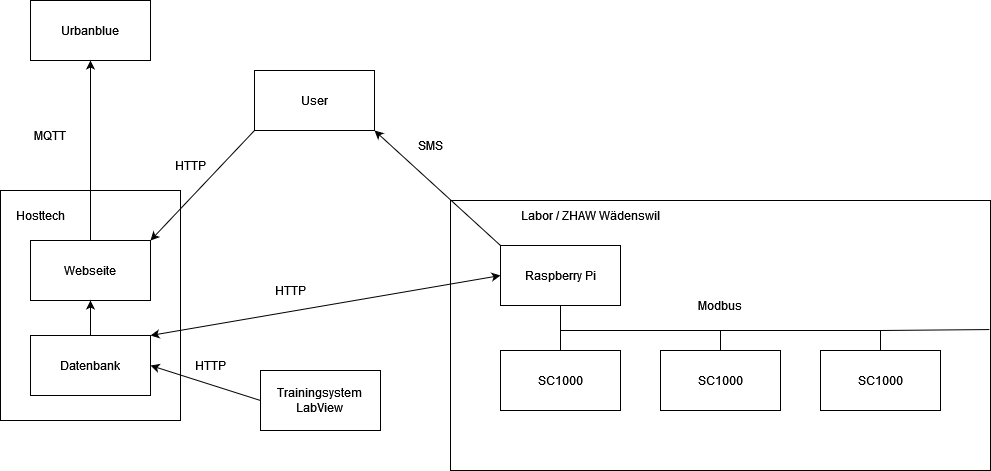
\includegraphics[scale=0.3]{pa_altes_system}
		\caption{Überblick aktuelles System}
		\label{fig:pa_altes_system}
	\end{figure}
	
	\subsection{Aufgabenstellung}
	Die Datenbank, in der die Sensordaten geloggt werden, besteht aus zwei Tabellen. In einer der Tabellen werden die Sensoren eingetragen, die sich in den Systemen befinden und in der zweiten Tabelle werden die Sensordaten abgespeichert und mit dem jeweiligen Sensor verknüpft. \\
	\\	
	Das Bearbeiten dieser Zuordnungstabelle ist für die Mitarbeiter/Studierende der ZHAW Life Sciences und Facility Management mit dem von Hosttech gegebenen Tool «phpMyAdmin» nicht verständlich. Zusätzlich müssen spezifische Werte eingegeben werden die einen Informatik Laien nicht bekannt sind, welches zu inkorrekte Angabe von Daten führen kann, welches wiederum zu einem Durcheinander in der Log-Tabelle führt. 
	Das «phpMyAdmin» Tool ist ebenfalls nur per Verwaltungsseite der Hosttech Domain erreichbar welches eine zusätzliche Hürde darstellt.
	
	\subsection{Zielsetzung}
	Um die Zuordnuntabelle einfacher zu bearbeiten, soll der Ablauf abgändert werden. Als Lösung stellen wir eine REST Schnittstelle zur Verfügung über welche die Tabelle mit wenigen Handgriffen verändert werden kann. 
	Diese soll übersichtlich und einfach zu bedienen sein. Damit die Schnittstelle zu jeder Zeit erreichbar ist soll sie gehostet werden.
\end{document}